\chapter{Activity Protocols}

\section{Debugging Activity}
The debugging activity embedded assessment was scaffolded by a short lecture presented by the researcher. The following pages include the slides from that lecture, followed by a description of the starter app provided to the students, and then the student worksheet.
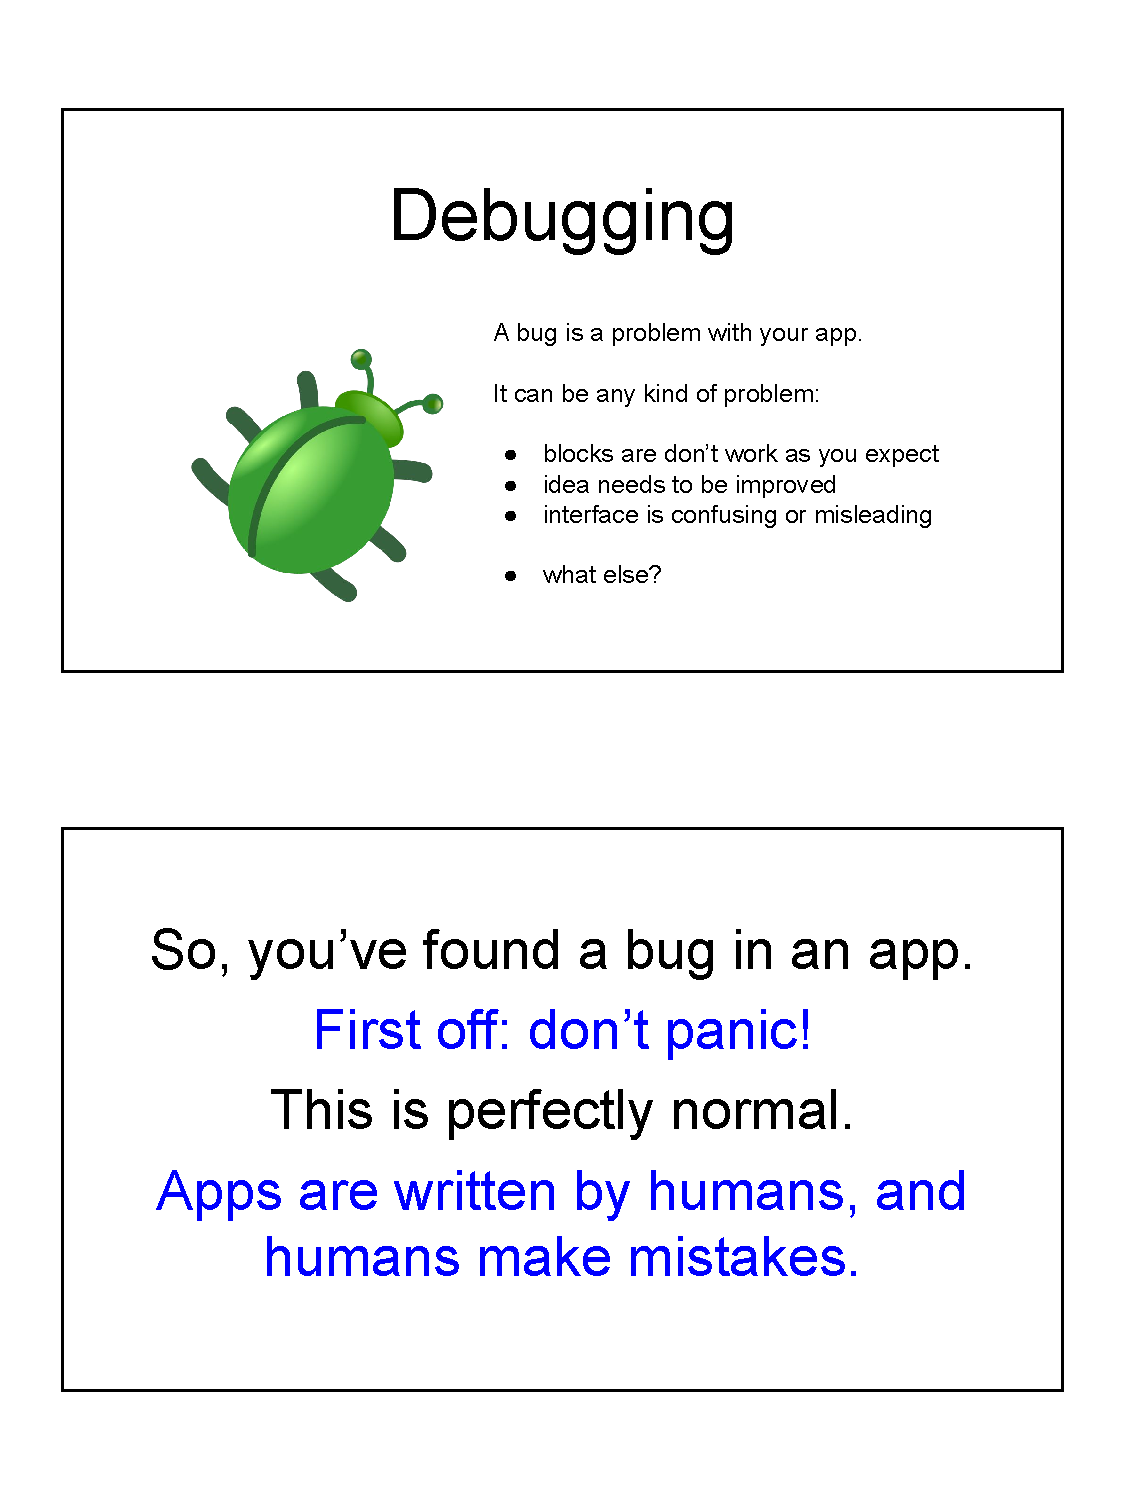
\includepdf[pages=-]{IRB/Mark_Debugging_Lecture_handout.pdf}
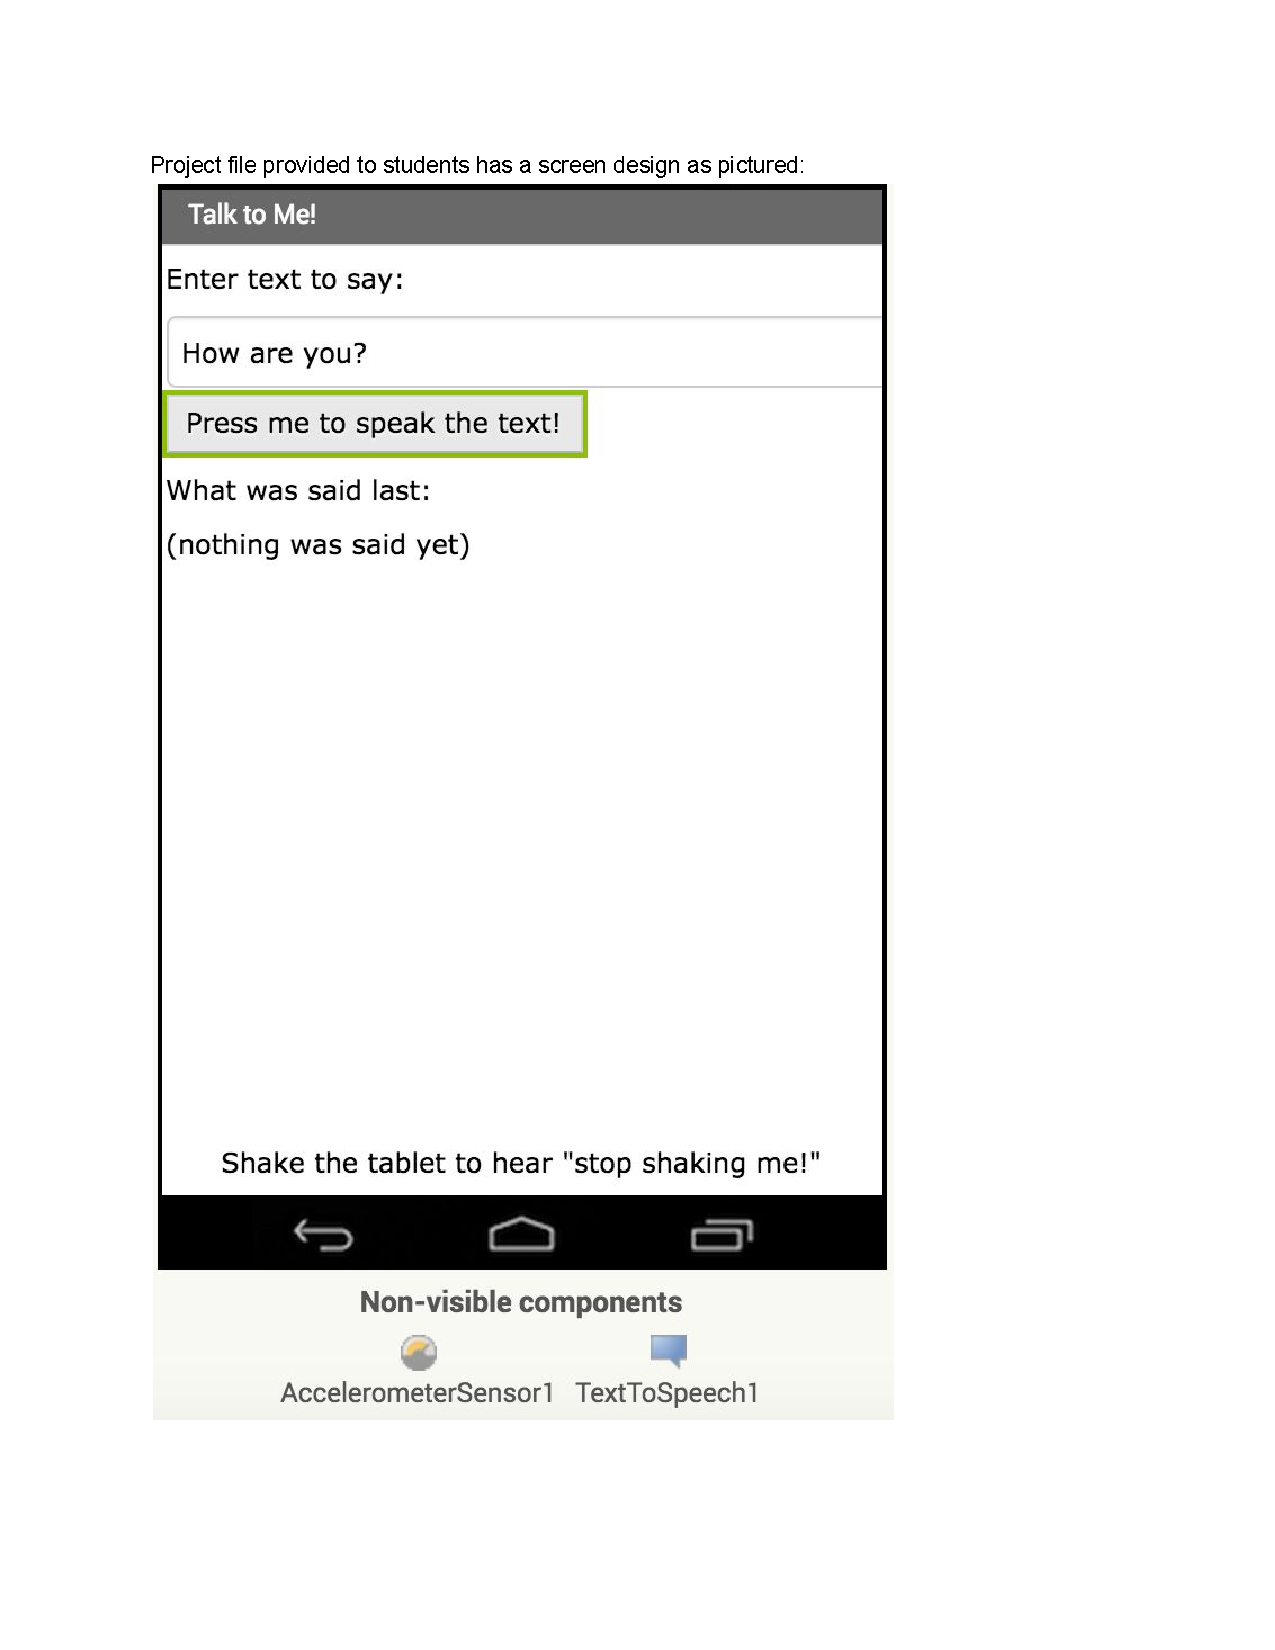
\includepdf[pages=-]{IRB/AM10DebuggingAssessment.pdf}
\label{apx:debugging-protocol}

\section{Temperature Activity}
The temperature activity embedded assessment was conducted during the summer camp. The following pages include a description of the starter app and the student worksheet. This activity did not have a slide deck to accompany its scaffolding lecture, and one needs to be added for future implementations.
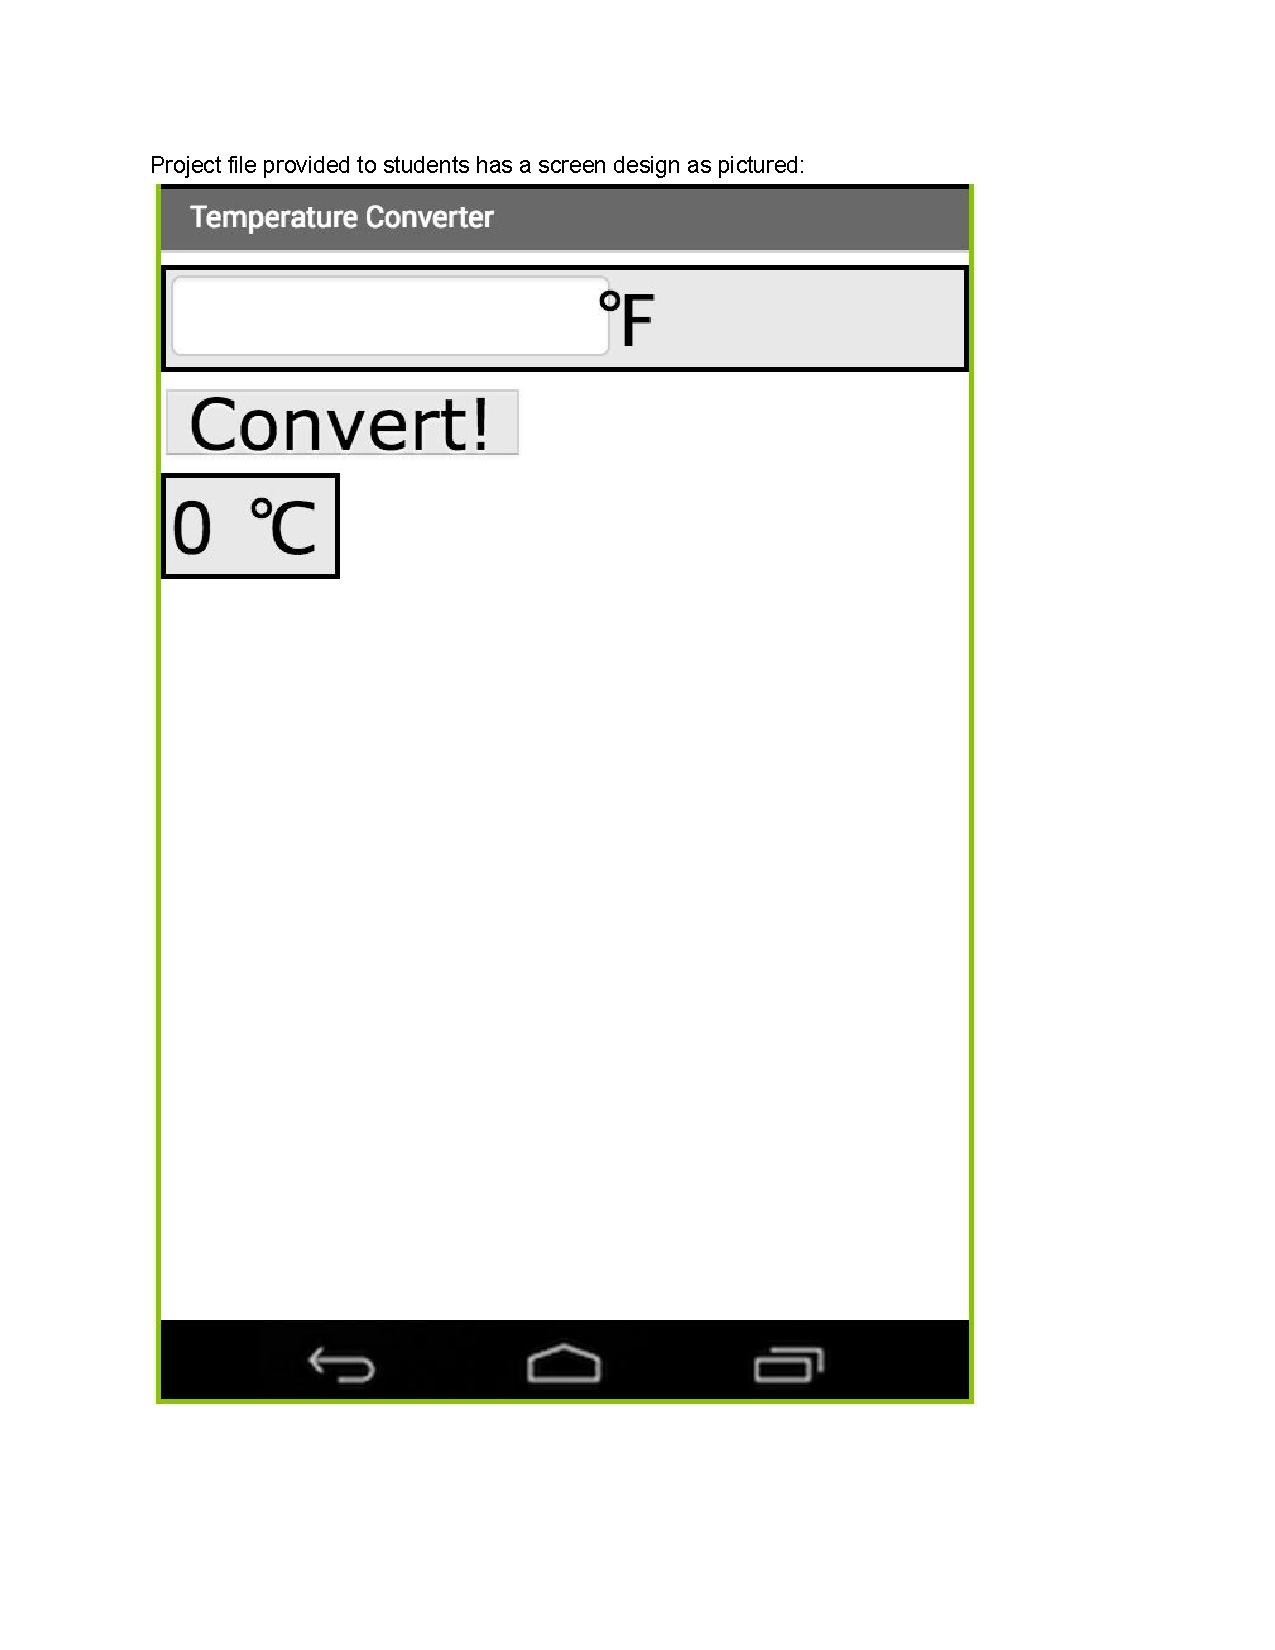
\includepdf[pages=-]{IRB/AM10TemperatureAssessment.pdf}
\label{apx:temperature-protocol}

\chapter{Institutional Compliance Forms}
This project was monitored by the UMass Lowell Office of Institutional Compliance Institutional Review Board (IRB). This section contains the relevant submissions and approval letters between the research team and the IRB.

% \section{IRB Application}
% \label{IRB:app}
% "Middle School Pathways in Computer Science" was originally submitted by Fred Martin on June 25, 2014. Approval was received after expedited review on July 7, 2014, as IRB Protocol \# 14-144-MAR-XPD. The approval period was for July 7, 2014 through July 6, 2015.

% The following pages contain a copy of the IRB application form and the approval letter in response.

% 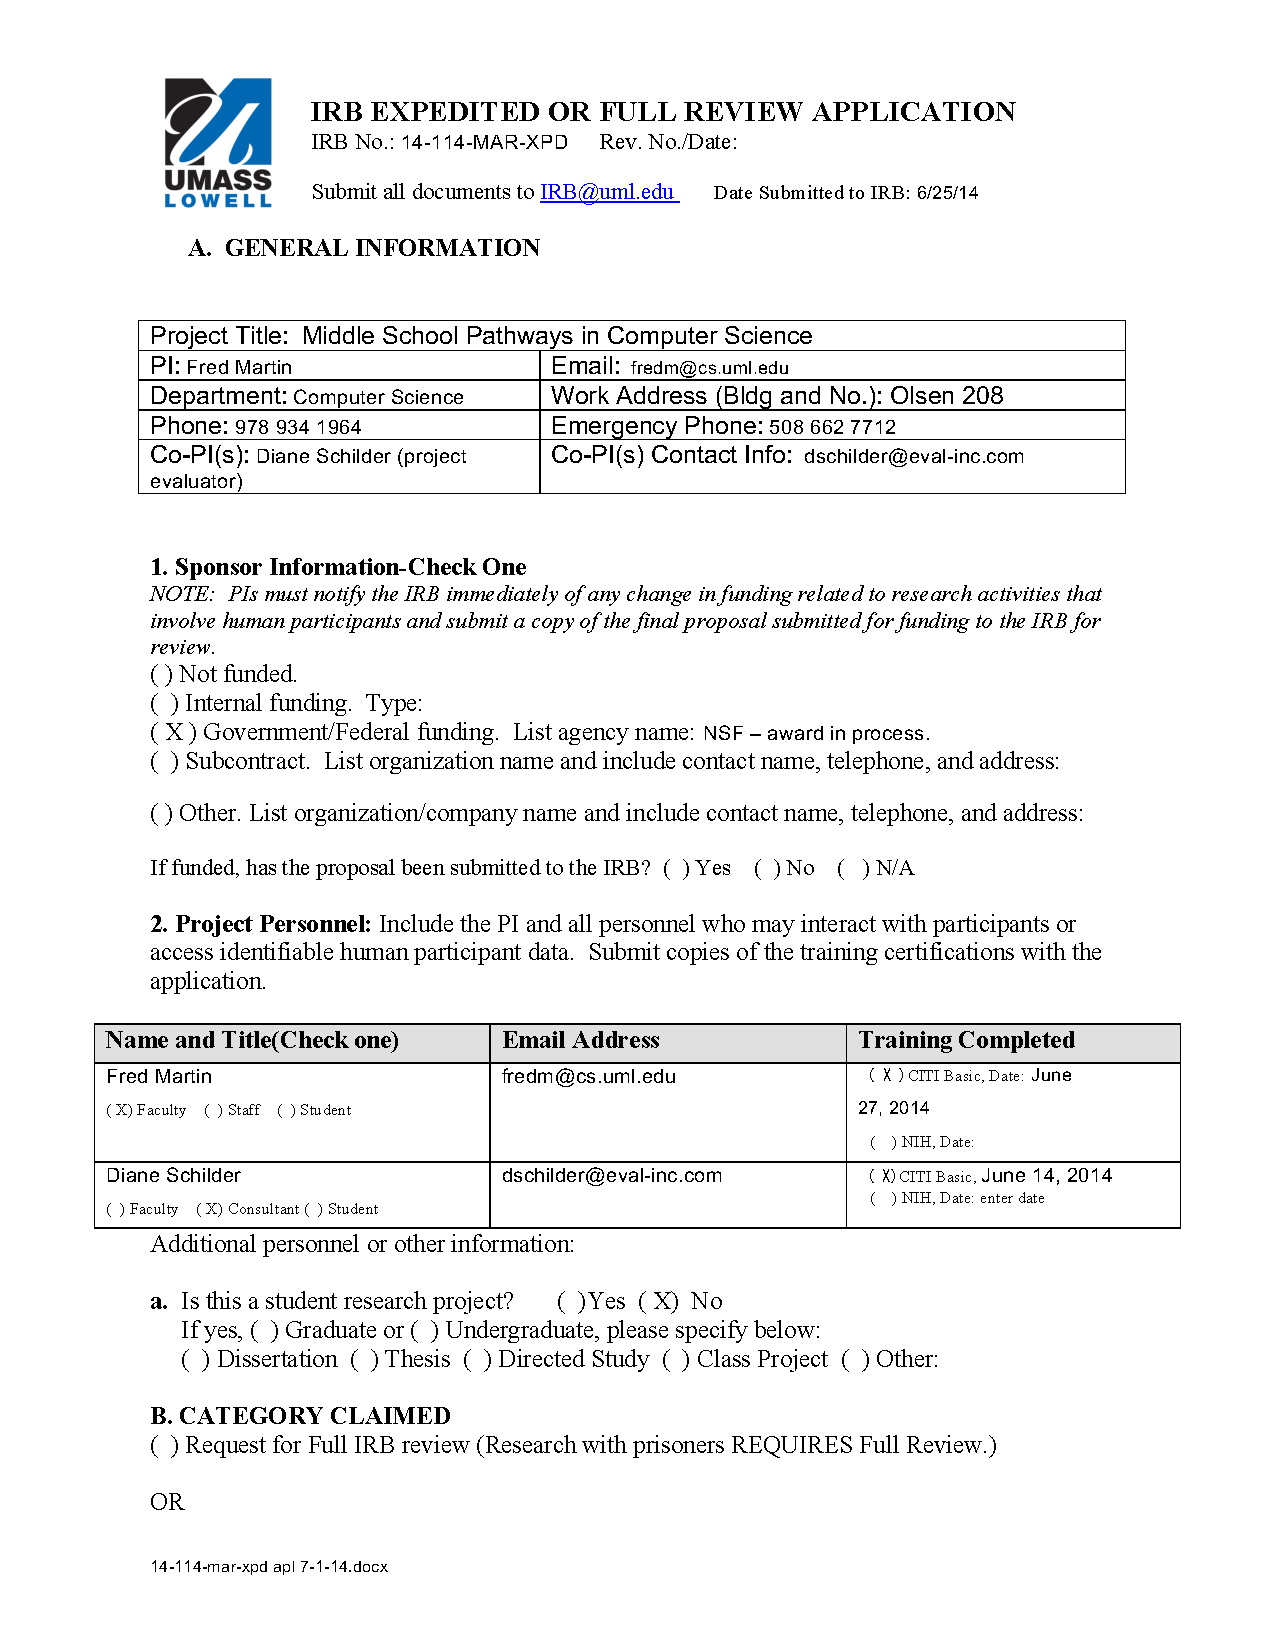
\includepdf[pages=-]{IRB/14-144-app.pdf}
% 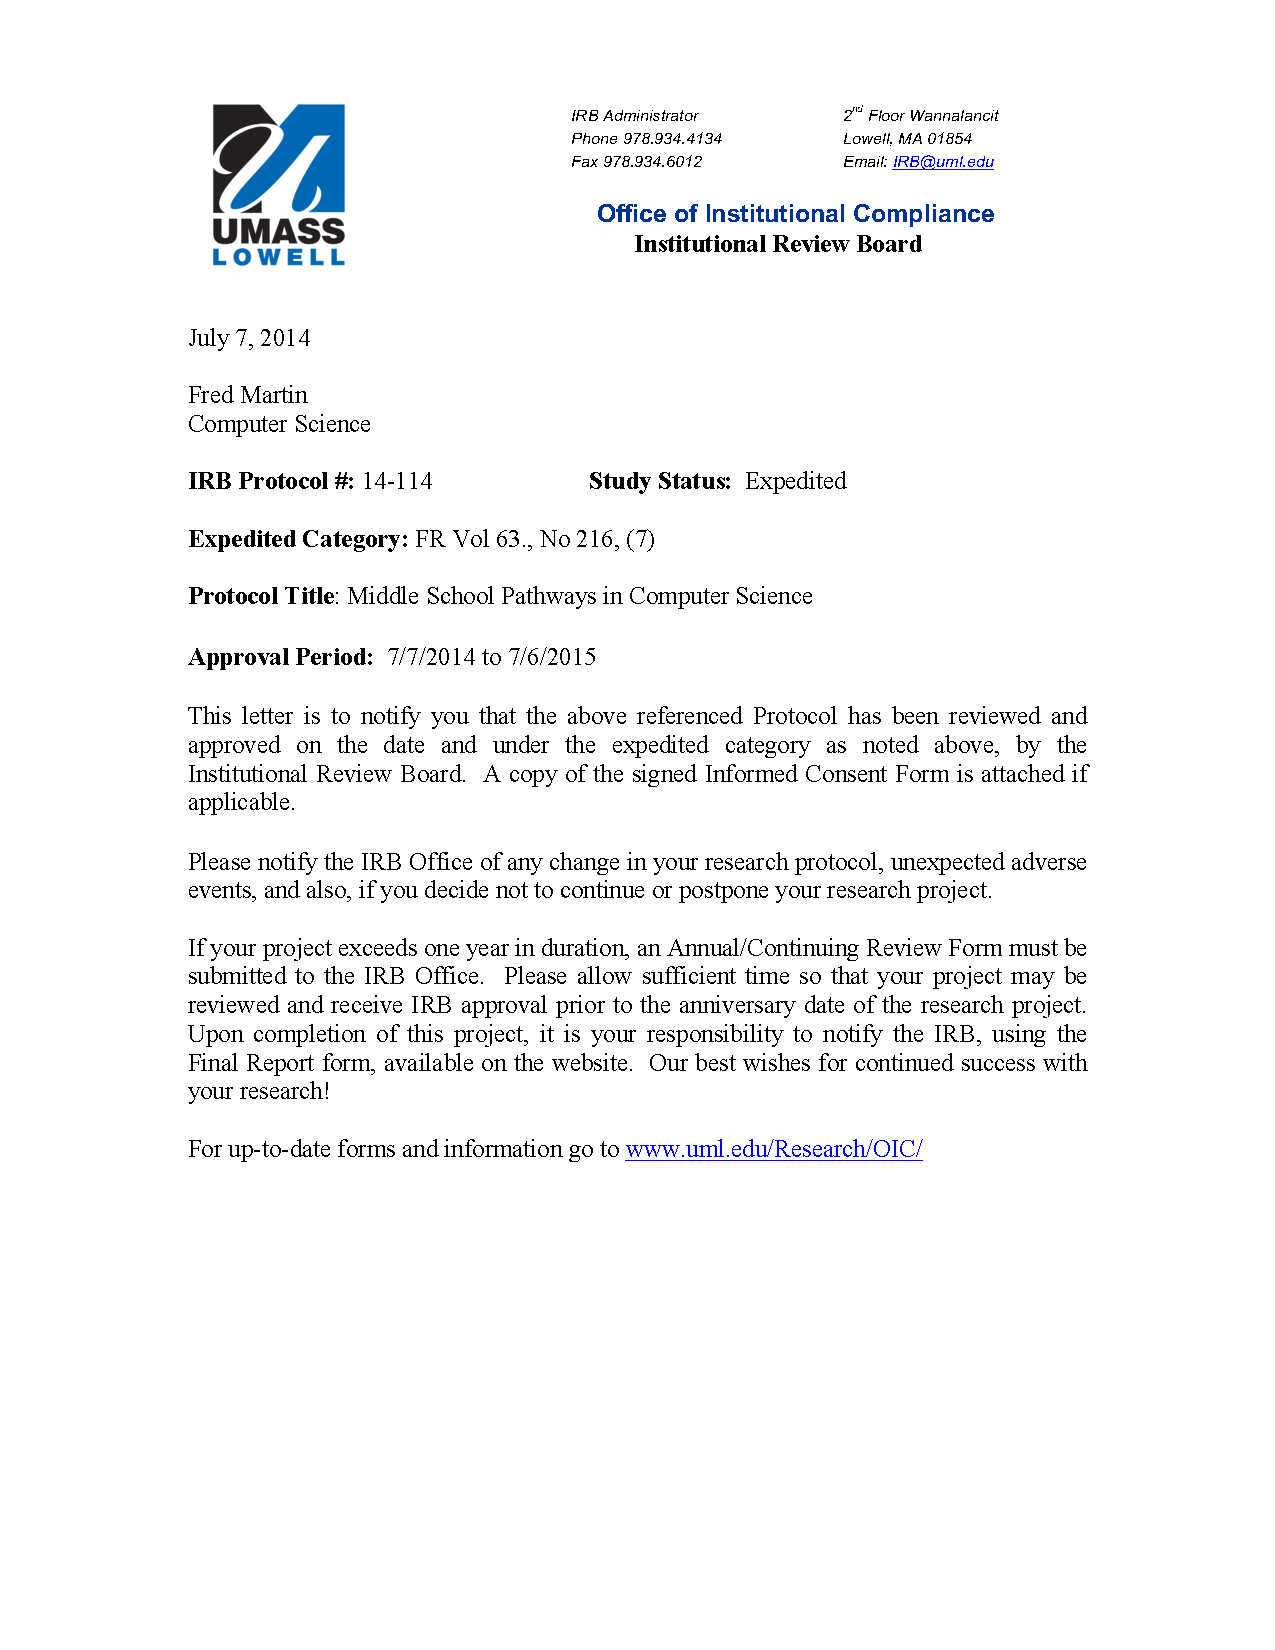
\includepdf[pages=-]{IRB/14-144-apv.pdf}

% \section{IRB Amendment 2}
% This amendment added the author, Mark Sherman, and fellow researcher Lijun Ni to the project. This amendment also specified the Debugging Activity, and its protocol for classroom use, which are shown in Appendix \ref{app:debug-protocol}. This amendment included the data de-identification protocol, which is discussed in Section \ref{sec:deident}.

% The following pages contain the Debugging Game protocol description, including the de-identification protocol, a copy of the amendment application, and the approval letter.

% 
\includepdf[pages=-]{IRB/AM2-DebuggingActivity2015.pdf}
% 
\includepdf[pages=-]{IRB/AM2-application.pdf}
% 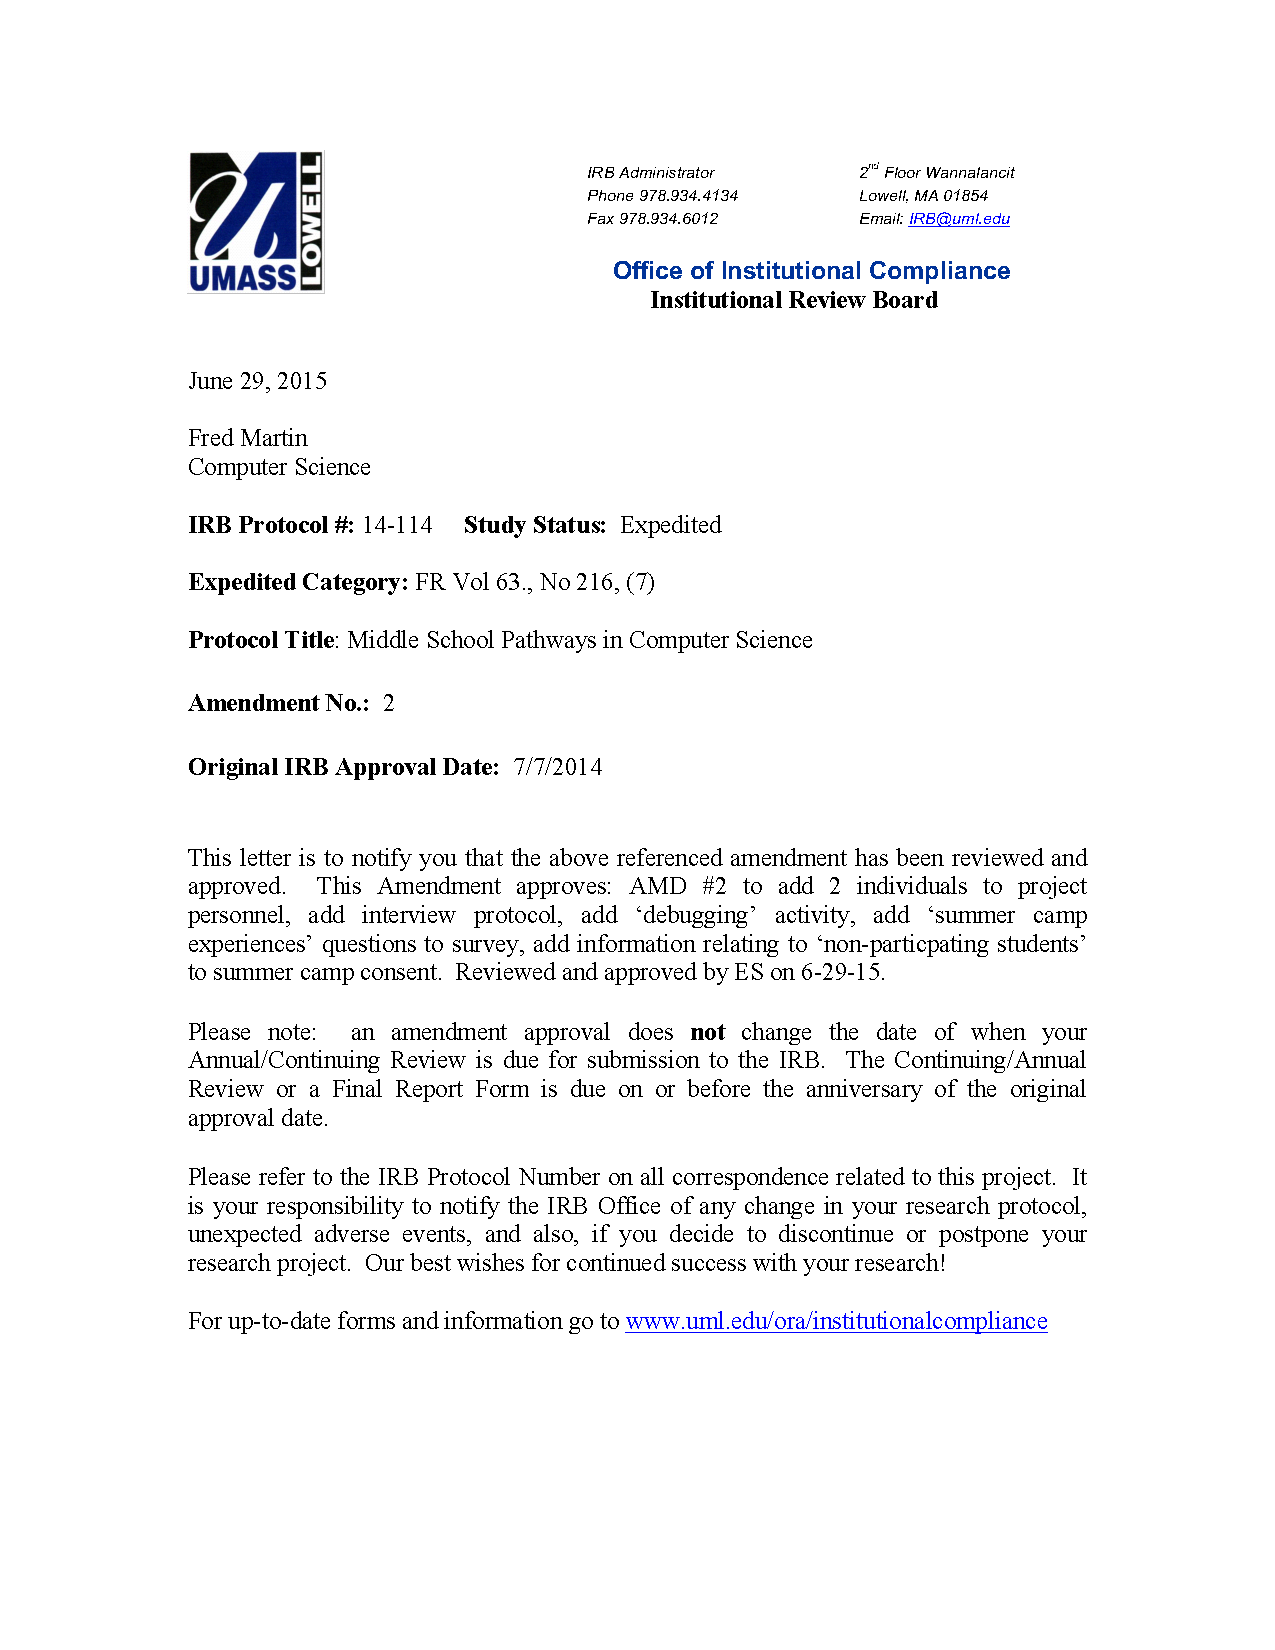
\includepdf[pages=-]{IRB/AM2-approve.pdf}
% \label{IRB:deident}


% \section{Annual/Continuing Review 2015}
% This application updated the IRB on the activities of the first year of the grant project, and declared intent for ongoing participant recruitment and data analysis until August 31, 2017. The following pages contain a copy of the review application and approval letter. The letter also mentions Amendment 3, which was approved at the same time, but is not relevant to the research in this document.

% 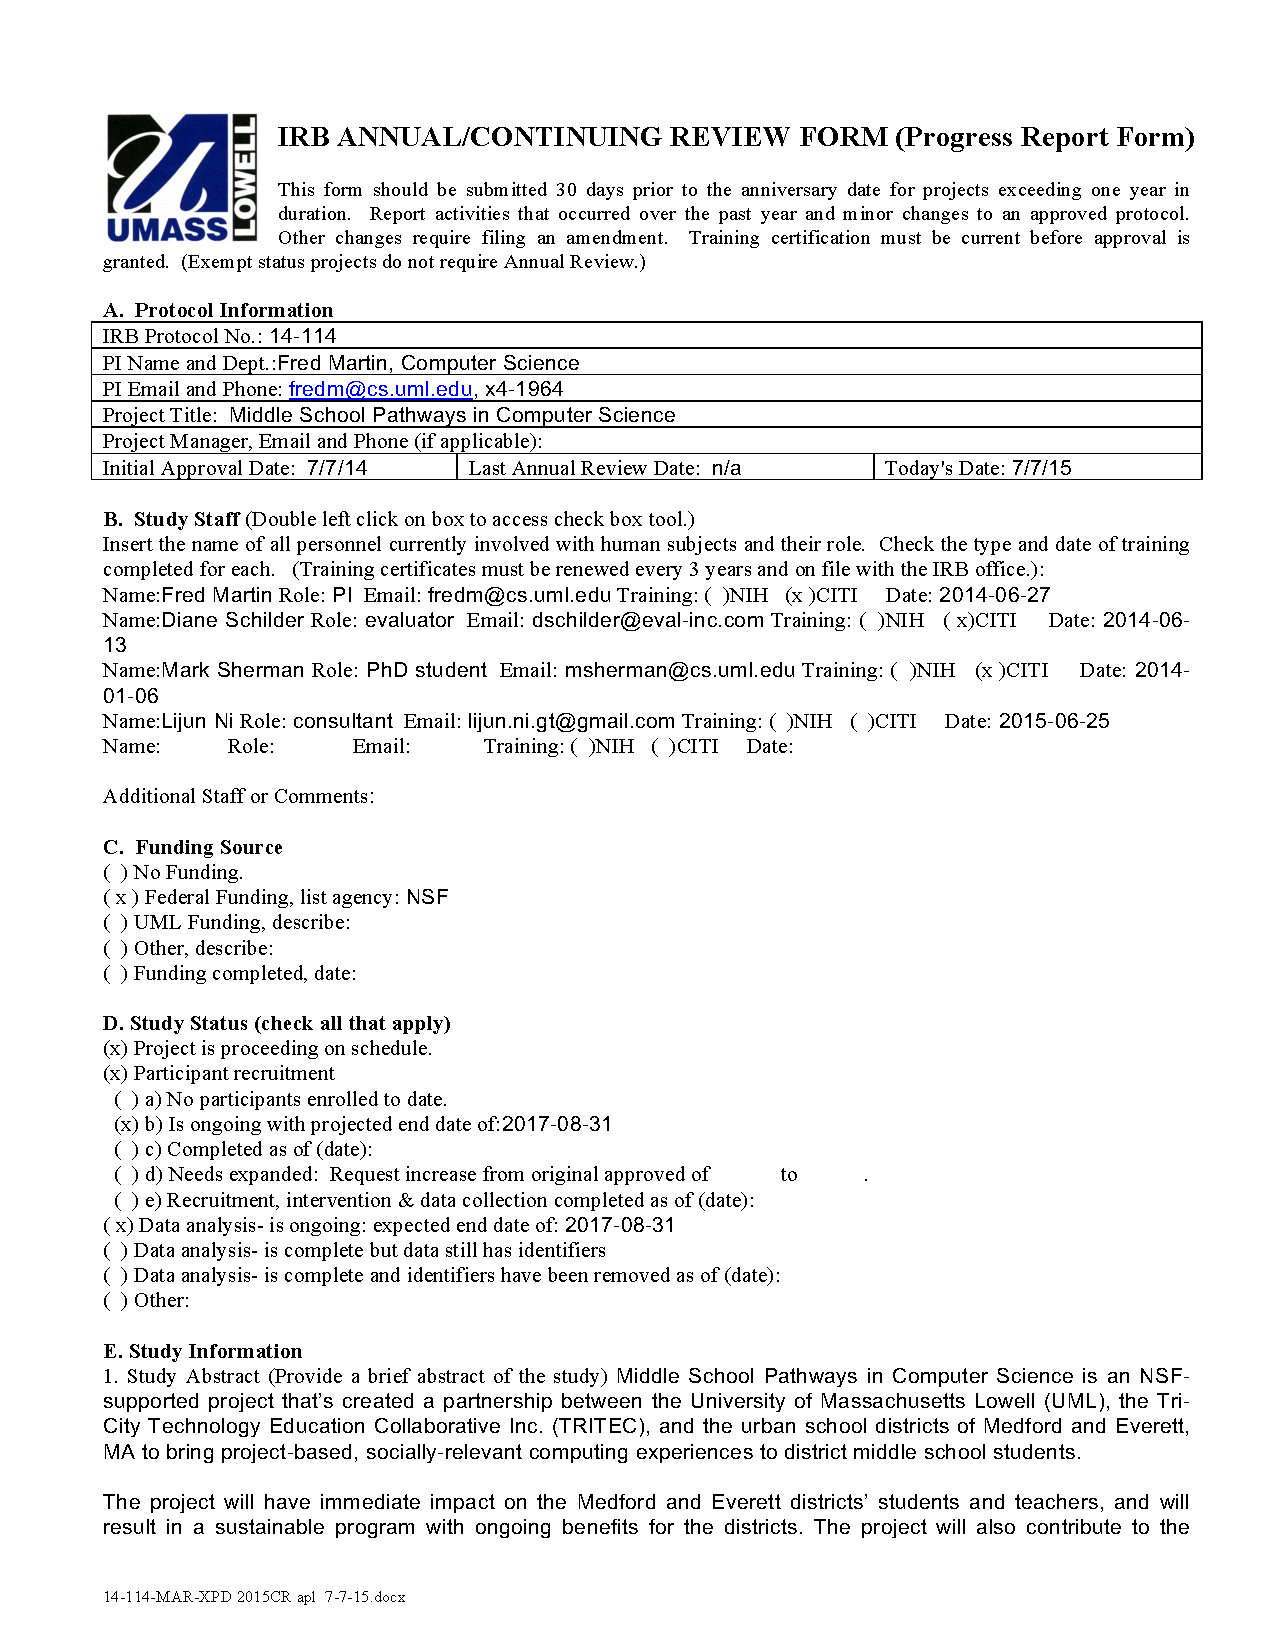
\includepdf[pages=-]{IRB/Year1-review-apl.pdf}
% 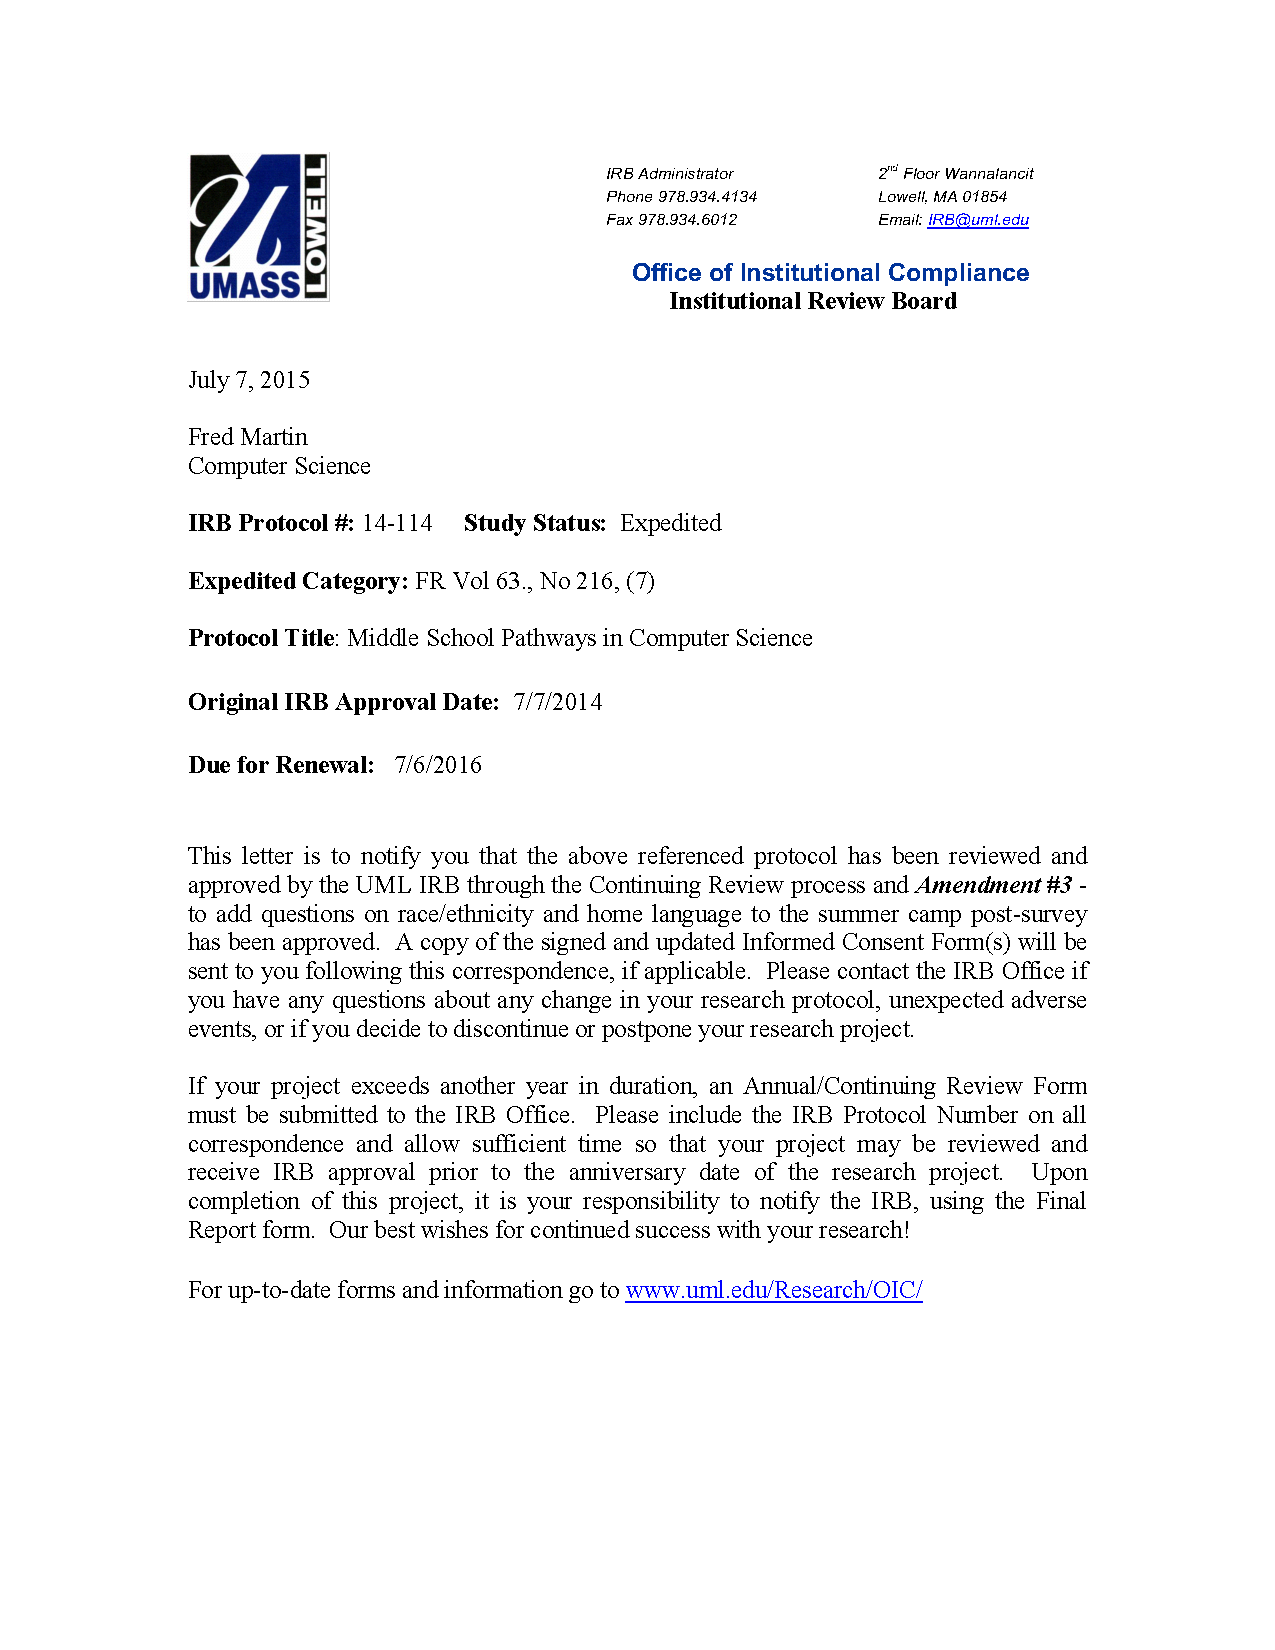
\includepdf[pages=-]{IRB/Year1-review-apv.pdf}

\section{Informed Consent, In-School}
\label{sec:icf:school}
The participants in this study were children, so an informed consent form was created for their parents, and a student assent form was provided to the children. The following pages are copies of those consent and assent forms as they were presented to the in-school cohort.

\includepdf[pages=-]{IRB/icf-parent-in-school-rev3-9-14-15.pdf}
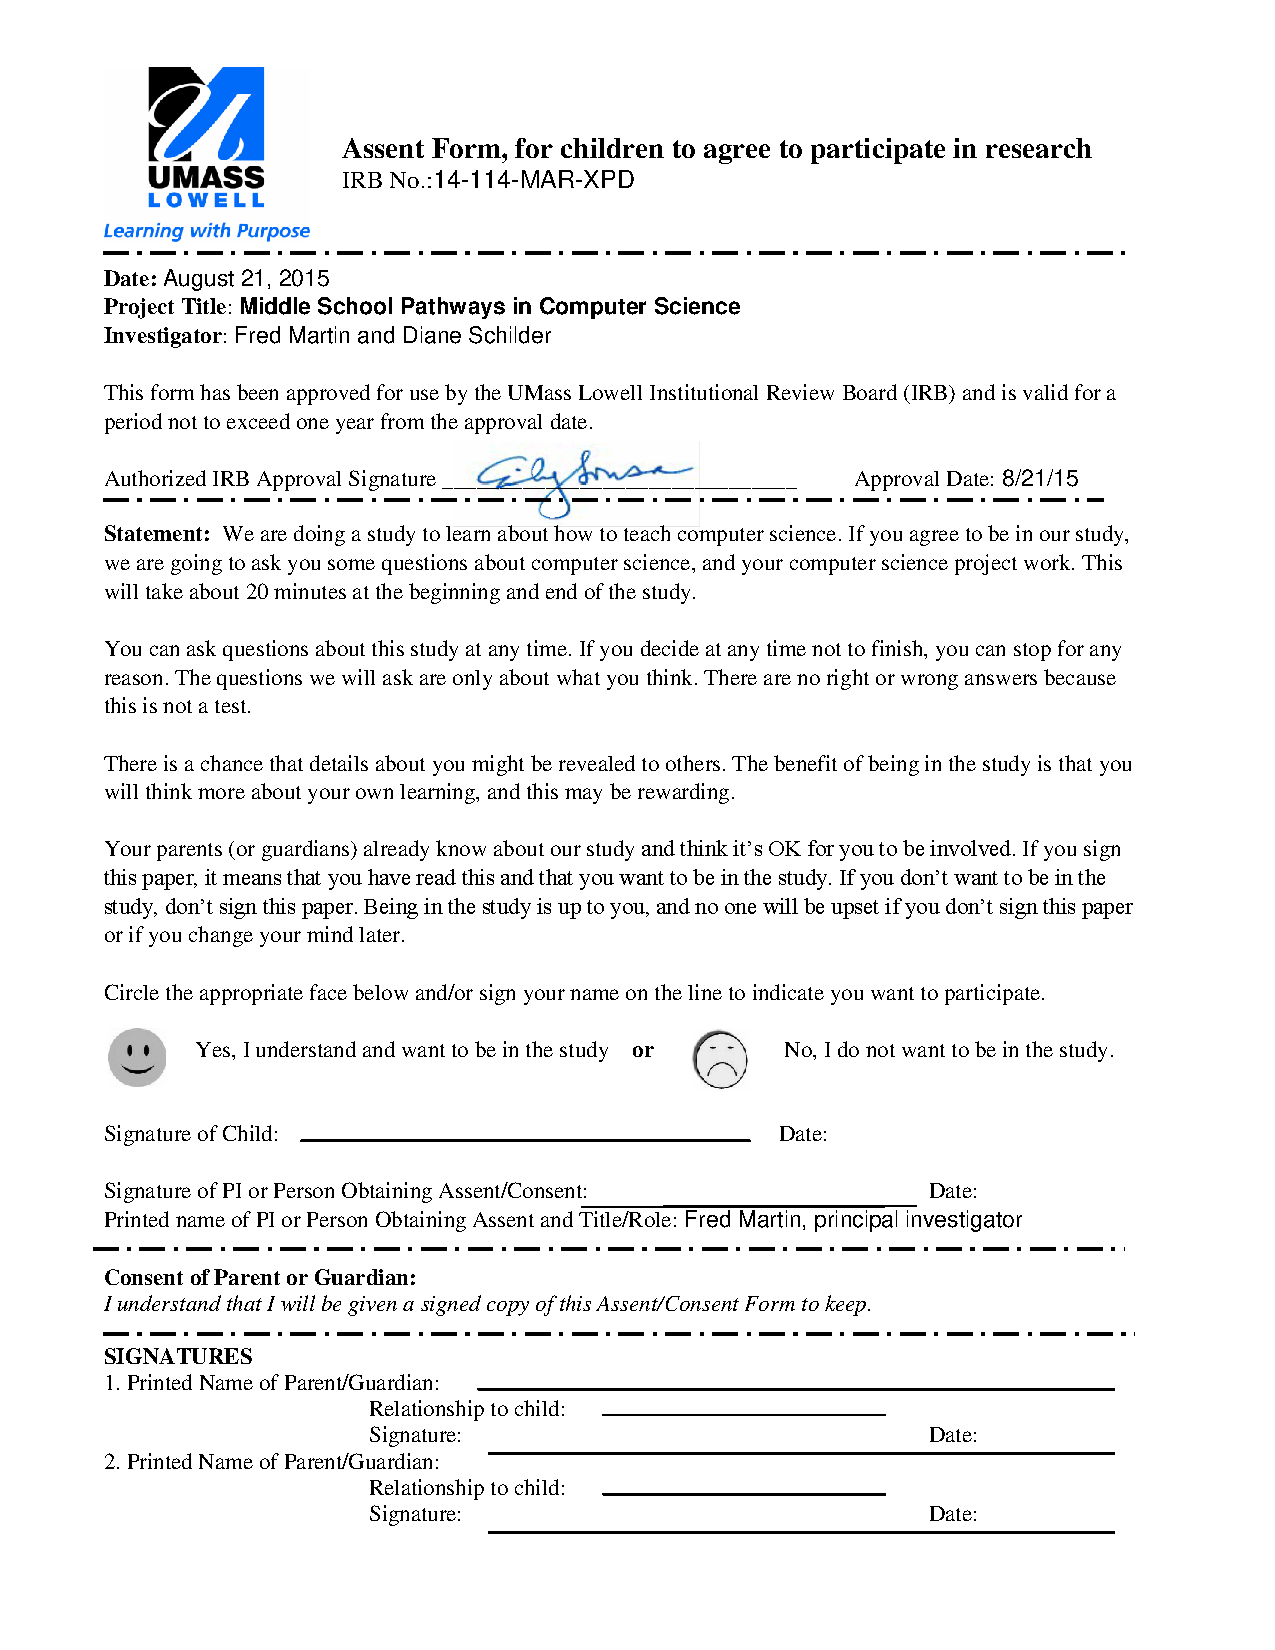
\includepdf[pages=-]{IRB/icf-assent-8-21-15.pdf}


\section{Informed Consent, Summer Camp}
\label{sec:icf:camp}
The participants in this study were children, so an informed consent form was created for their parents, and a student assent form was provided to the children. The student assent form was unchanged from the In-School cohort (Appendix \ref{sec:icf:school}). The parental consent form was updated. The following pages are copies of the updated summer camp parental consent and the corresponding IRB approval letter.


\includepdf[pages=-]{IRB/icf-summer-camp-parent-consent-2016.pdf}
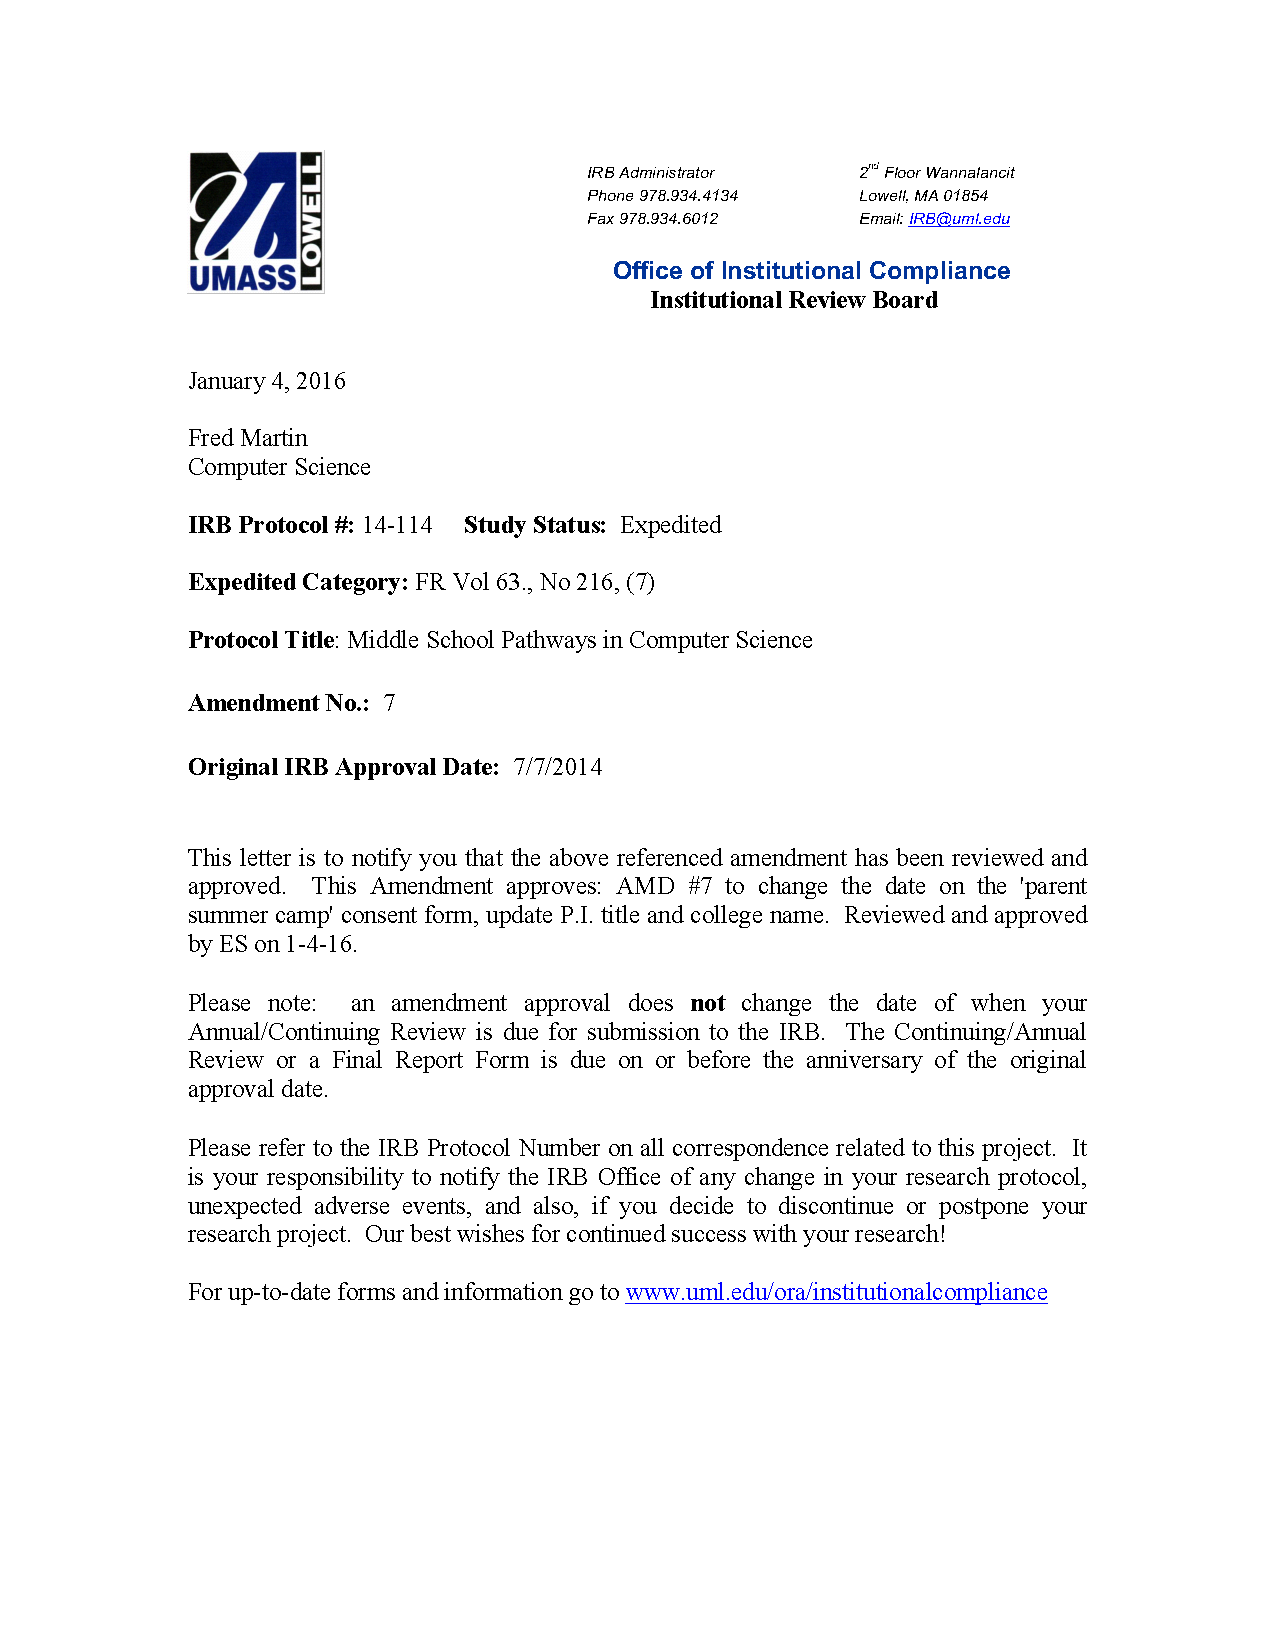
\includepdf[pages=-]{IRB/icf-summer-camp-parent-consent-2016-approval.pdf}


% \section{Student Activities for Summer Camp Research}
% Amendment 10 added protocols for the Debugging Activity and Temperature Activity, both of which were used for data collection in this research. The protocol documents follow in Sections \ref{sec:IRB:debugging} and \ref{sec:IRB:temperature}, respectively. The following pages are copies of the IRB amendment form, and the approval letter affirming that these instruments operate under previously approved informed consent mechanisms. 

% 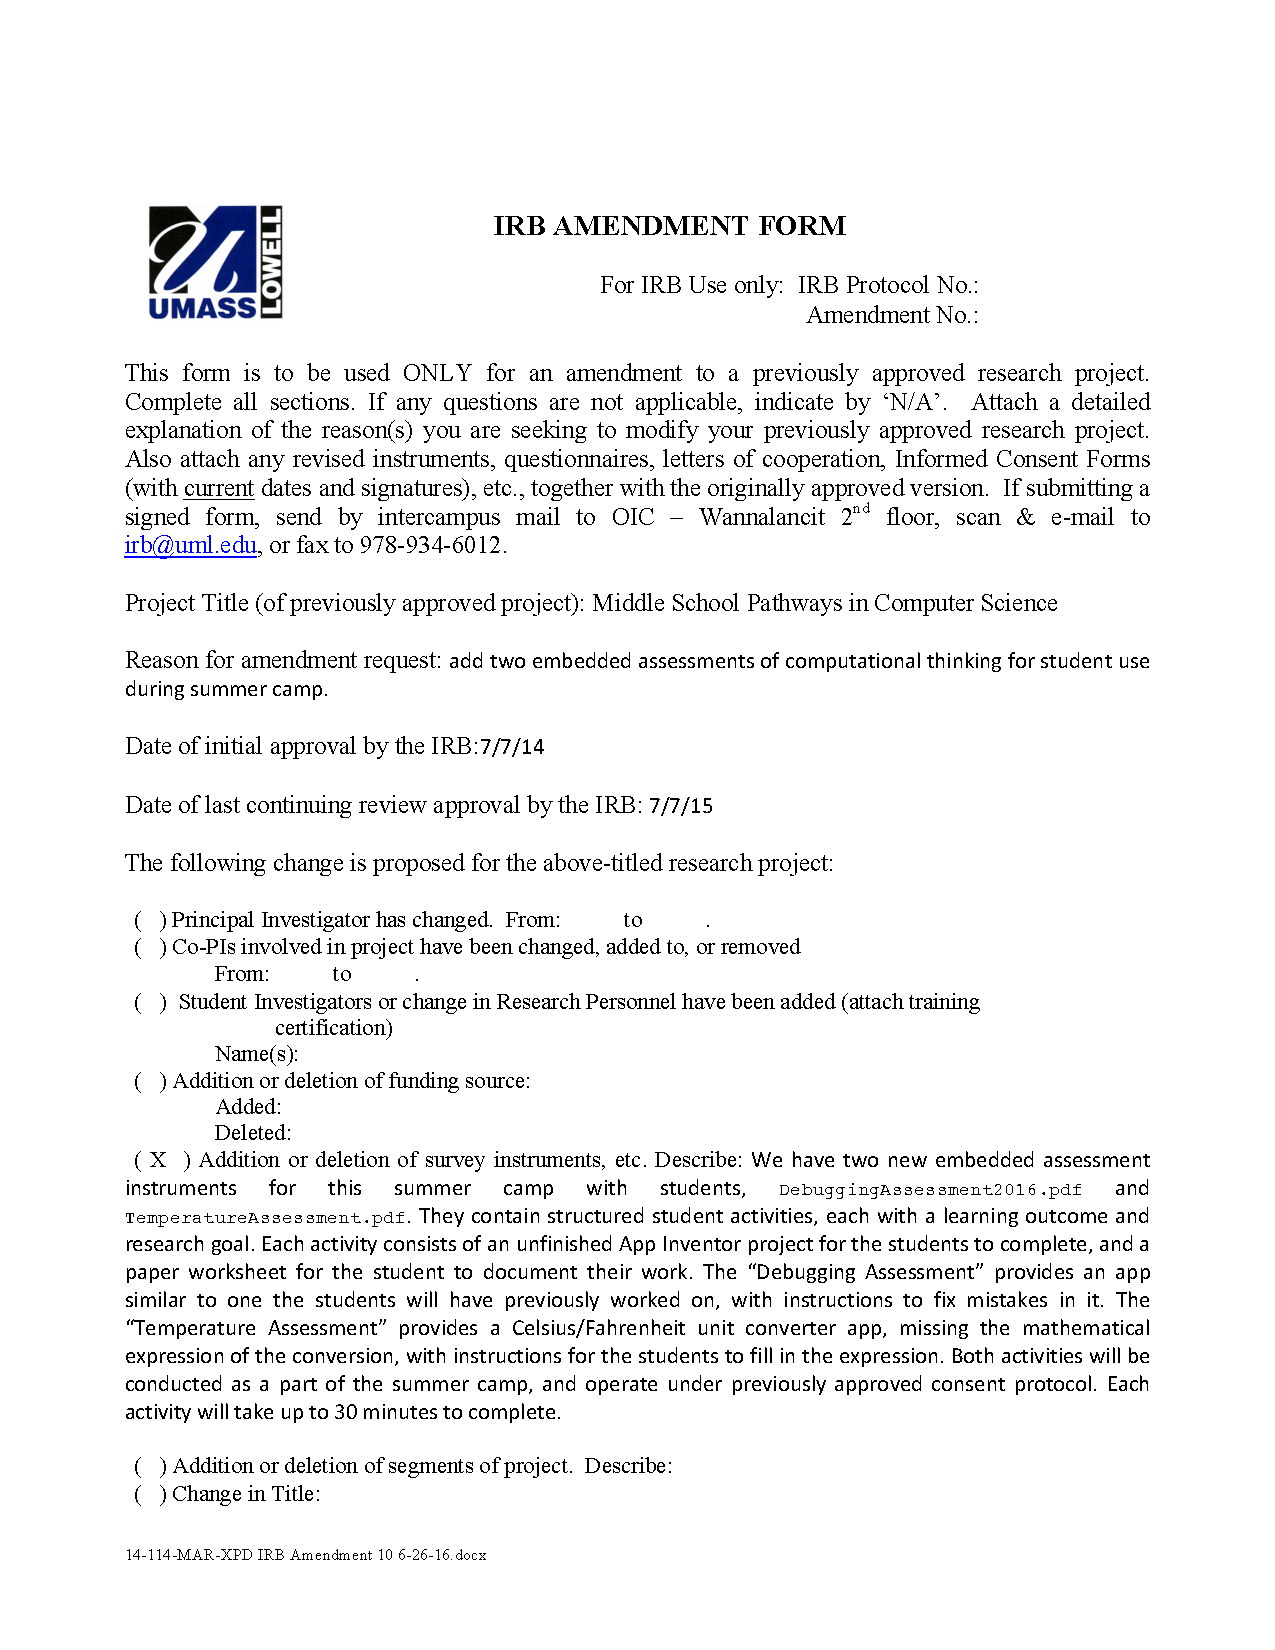
\includepdf[pages=-]{IRB/AM10-application.pdf}
% 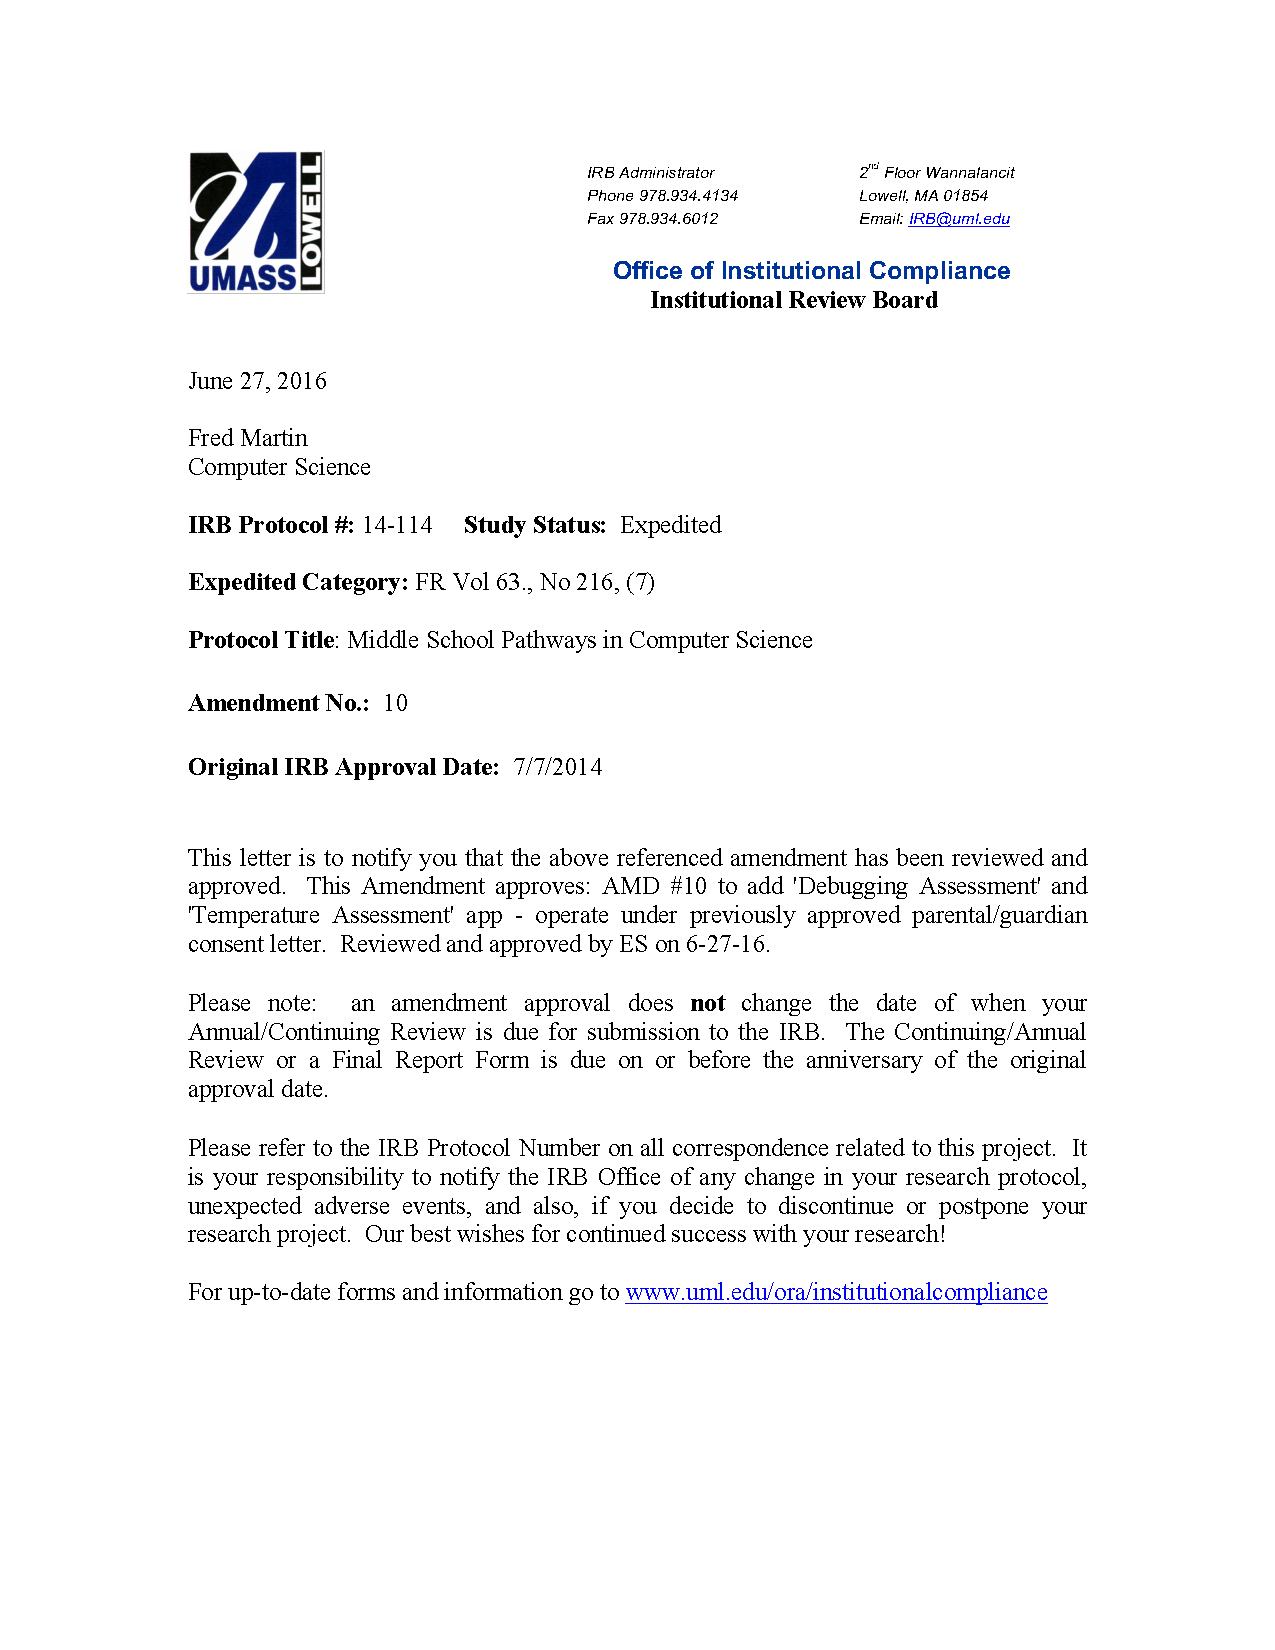
\includepdf[pages=-]{IRB/AM10-apv.pdf}



%%%%%%%%%%%%%%%%%%%%%%%%%%%%%%%%%%%%%%%%%%%%%%%%%%%%%%%%%%%%%%%%%%%%%%%%%%%%%%%%
%%%%%%%%%%%%%%%%%%%%%%%%%%%%%%%%%%%%%%%%%%%%%%%%%%%%%%%%%%%%%%%%%%%%%%%%%%%%%%%%

\chapter{Code Availability}

\noindent The App Inventor project, supported by the MIT Center for Mobile Learning, can be found here:

\noindent \url{https://github.com/mit-cml/appinventor-sources}

\noindent The modified version of App Inventor used in this project can be found in the author's github account:

\noindent \url{https://github.com/marksherman/appinventor-sources/tree/snapshot-service}

\noindent The long-term home for the features from this project is within the github home of the Engaging Computing Lab at UMass Lowell. That code can be found here:

\noindent \url{https://github.com/engaging-computing/appinventor-sources}

\noindent The source of this document is available from the author here:

\noindent \url{https://github.com/marksherman/umlthesis/tree/markphd}

\noindent The template used to write this document is available from the Engaging Computing lab at UMass Lowell:

\noindent \url{https://github.com/engaging-computing/umlthesis}

%\noindent Especially relevant excerpts from the source code are listen in Appendix \ref{appendix:listings}.

%\chapter{Code Listings} \label{appendix:listings}

%Interesting source code for the data capture, collection, and analysis systems used in this project are listed in full here. All code was written by the author except where noted.

% font sizes, ascending: \tiny \scriptsize \footnotesize \small \normalsize
% scriptsize gets a little more than 80 chars wide and 44 lines on the page, which is fair.
\setminted{fontsize=\scriptsize, fontfamily=courier, linenos, breaklines}


% \section{Modifications to App Inventor}
% \label{src:appinventor}

% \subsection{snapshot.js}
% \label{src:ai/snapshot.js}
% This file was added to the blockly editor within App Inventor, and provided the snapshot collection and transmission features. The public function is \emph{Blockly.Snapshot.send,} which was called elsewhere in blockly to trigger a snapshot. As listed below, the feature will connect to a local test server. For production, the comments on line 13 and 14 were swapped, allowing connection to the real data collection server. 
% \inputminted{javascript}{src/appinventor/snapshot.js}

% \subsection{Modifications to BlocklyPanel.java}
% \label{src:ai/BlocklyPanel.java}
% This file provided the interface between the general App Inventor web page, including the Designer, and the javascript blockly environments. The page and Designer were composed using the Google Web Toolkit (GWT), which was written in Java and compiled to javascript. The snapshot mechanism was implemented in the blockly environment, in pure javascript, but required access to certain data in the GWT environment. Modifications to this file exposed that data to blockly, and the snapshot system, as seen in the file excerpts below.

% \inputminted[firstline=626, lastline=651]{java}{src/appinventor/BlocklyPanel.java}
% \inputminted[firstline=902, lastline=913, breakbefore=.]{java}{src/appinventor/BlocklyPanel.java}


% \section{Snapshot Receiver Service}
% \label{src:snapshot-service}
% The Snapshot Service was the server-side receiving mechanism that de-identified and stored snapshots generated by App Inventor. This service was written in javascript for node.js.

% \subsection{file.js}
% \label{src:file.js}
% RPC module that implements the \emph{file.saveProject} API endpoint. It takes raw snapshot data, applies the de-identifier, and saves the snapshot to disk.
% \inputminted{javascript}{src/snapshot-service/file.js}

% \subsection{userdb.js}
% \label{src:userdb.js}
% De-identifies user names, replacing them with unique code names, and stores the relationship in a database.
% \inputminted{javascript}{src/snapshot-service/userdb.js}

% \subsection{savegit.js}
% \label{src:savegit.js}
% Provides utilities to interface with git on the server to save data. Each user's project is represented by a git repository, and each snapshot creates a new commit in that repository. This is used by file.js.
% \inputminted{javascript}{src/snapshot-service/savegit.js}

% \subsection{gc.sh}
% \label{src:gc.sh}
% The additive git method used by this service creates inefficiencies on the host file system that consumes space and inodes at a high rate. This script `garbage collects' the database, repacking it efficiently, and should be run occasionally while the system is in use. This file is included here as a warning to anyone in the future who wants to use git as a database.
% \inputminted{bash}{src/snapshot-service/gc.sh}


% \section{Analysis Tools}

% \subsection{main.py}
% %TODO This needs to be updated when the scrips change! Make sure this is re-copied latex directory before final thesis print!
% This is currently an in-progress version of this file, containing provisional scratchwork and some in-development modifications. These temporary features will be removed and replaced with restored, fully consistent code for the final dissertation document.
% \inputminted[lastline=212]{python}{src/analysis/main.py}

% \subsection{gitfilter.py}
% \inputminted[lastline=168]{python}{src/analysis/gitfilter.py}
% \subsection{xml\_analyze.py}
% \inputminted[lastline=261]{python}{src/analysis/xml_analyze.py}


% \section{Snapshot Playback}
% The playback mechanism allowed a full history of snapshots from a project to be viewed in an App Inventor blockly window. It enabled the researcher to step through the history- forward, backwards, and arbitrarily, displaying the code blocks as the user placed them. Additionally the mechanism displayed the timestamp of the current snapshot, in seconds since the project was created, how many snapshots were taken, and what number snapshot was currently being viewed.

% This file, \emph{playback.js,} was added to the blockly editor within App Inventor, and provided the playback feature. It used the javascript console to start and control playback.
% \label{src:playback.js}
% \inputminted{javascript}{src/playback/playback.js}
